\section{Y86-64顺序处理器设计}
\begin{center}
    (该章满分50分)
\end{center}

\subsection{Y86-64顺序处理器结构设计}

\begin{figure}[H]
\centering
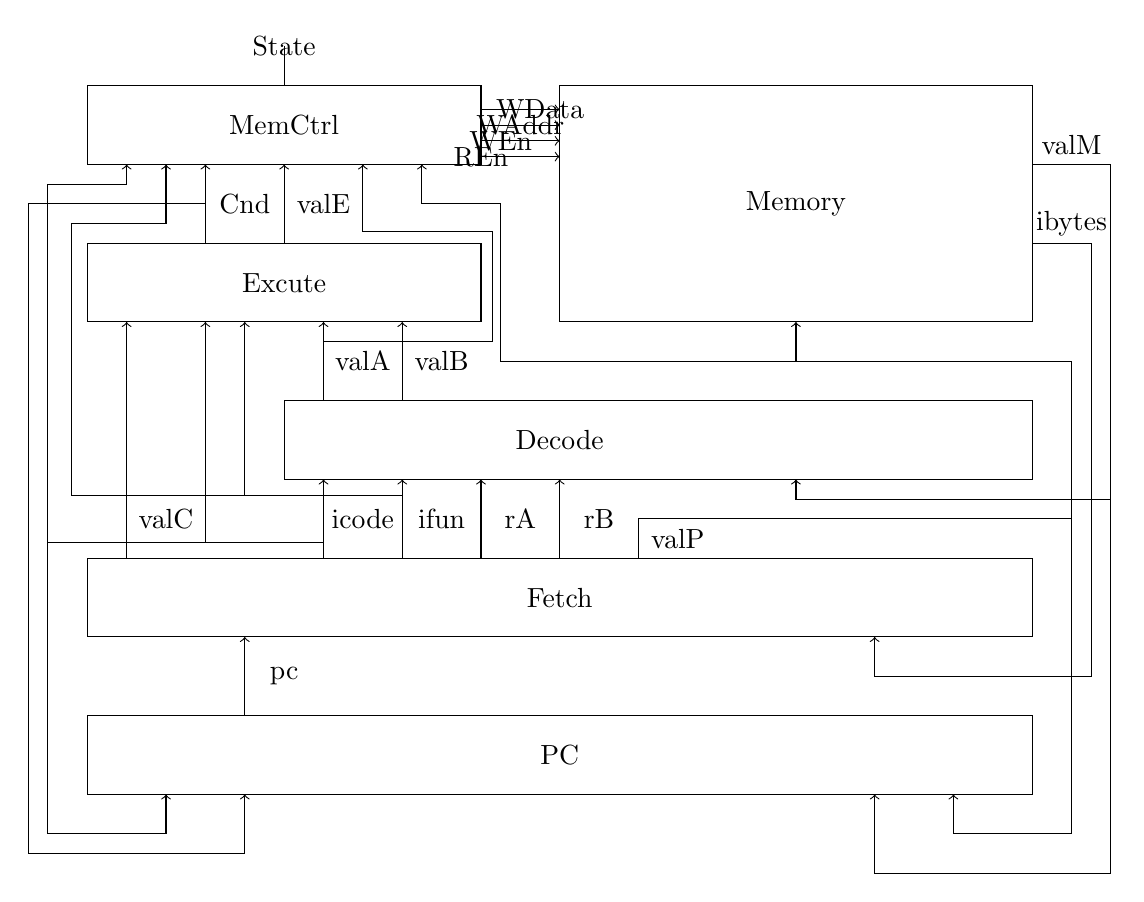
\begin{tikzpicture}
    \draw (0,0) rectangle +(12,1);
    \draw (6,0.5) node{PC};
    
    \draw (0,2) rectangle +(12,1);
    \draw (6,2.5) node{Fetch};
    
    \draw (2.5,4) rectangle +(9.5,1);
    \draw (6,4.5) node{Decode};
    
    \draw (0,6) rectangle +(5,1);
    \draw (2.5,6.5) node{Excute};
    
    \draw (0,8) rectangle +(5,1);
    \draw (2.5,8.5) node{MemCtrl};
    
    \draw (6,6) rectangle +(6,3);
    \draw (9,7.5) node{Memory};

%pc
    \draw [->](2,1) -- (2,2);
    \draw (2.5,1.5) node{pc};
    
%fetch
    \draw [->](3,3) -- (3,4);
    \draw [->](3,3.2) -- (1.5,3.2) -- (1.5,6);
    \draw [->](3,3.2) -- (-0.5,3.2) -- (-0.5,-0.5) -- (1,-0.5) -- (1,0);
    \draw [->](-0.5,3.2) -- (-0.5,7.75) -- (0.5,7.75) -- (0.5,8);
    \draw (3.5,3.5) node{icode};
    
    \draw [->](4,3) -- (4,4);
    \draw [->](4,3.8) -- (2,3.8) -- (2,6);
    \draw [->](4,3.8) -- (-0.2,3.8) -- (-0.2,7.25) -- (1,7.25) -- (1,8);
    \draw (4.5,3.5) node{ifun};
    
    \draw [->](5,3) -- (5,4);
    \draw (5.5,3.5) node{rA};
    
    \draw [->](6,3) -- (6,4);
    \draw (6.5,3.5) node{rB};
    
    \draw [->](0.5,3) -- (0.5,6);
    \draw (1,3.5) node{valC};
    
    \draw [->](7,3) -- (7,3.5) -- (12.5,3.5) -- (12.5,3.5) -- (12.5,-0.5) -- (11,-0.5) -- (11,0);
    \draw [->](12.5,3.5) -- (12.5,5.5) -- (5.25,5.5) -- (5.25,7.5) -- (4.25,7.5)--(4.25,8);
    \draw [->](9,5.5)--(9,6);
    \draw (7.5,3.25) node{valP};
    
%decode
    \draw [->](3,5) -- (3,6);
    \draw [->](3,5.75) -- (5.15,5.75) -- (5.15,7.15) -- (3.5,7.15) -- (3.5,8);
    \draw (3.5,5.5) node{valA};
    
    \draw [->](4,5) -- (4,6);
    \draw (4.5,5.5) node{valB};
    
%execute
    \draw [->](1.5,7) -- (1.5,8);
    \draw [->](1.5,7.5) -- (-0.75,7.5) -- (-0.75,-0.75) -- (2,-0.75) --(2,0);
    \draw (2,7.5) node{Cnd};
    
    \draw [->](2.5,7) -- (2.5,8);
    \draw (3,7.5) node{valE};
    
%memctrl
    \draw [->] (5,8.1) -- (5.0,8.1)node{REn} -- (6,8.1);
    \draw [->] (5,8.3) -- (5.25,8.3)node{WEn} -- (6,8.3);
    \draw [->] (5,8.5) -- (5.5,8.5)node{WAddr} -- (6,8.5);
    \draw [->] (5,8.7) -- (5.75,8.7)node{WData} -- (6,8.7);
    \draw (2.5,9) -- (2.5,9.5) node{State};
    
%memory
    \draw [->] (12,7) -- (12.75,7) -- (12.75,1.5) -- (10,1.5)--(10,2);
    \draw (12.5,7.25) node{ibytes};
    \draw [->] (12,8) -- (13,8) -- (13,-1) --(10,-1) -- (10,0);
    \draw [->] (13,3.75)--(9,3.75)--(9,4);
    \draw (12.5,8.25)node{valM};

\end{tikzpicture}
\caption{Y86-64处理器结构}
\end{figure}

\subsection{Y86-64顺序处理器模块设计(包含Verilog模块接口设计)}

\subsubsection{PC}
\begin{minted}{verilog}
module PC(
    input clock,
    input  [3:0] icode,
    input  Cnd,
    input  [63:0] ValM,
    input  [63:0] ValC,
    input  [63:0] ValP,
    output reg[63:0] pc,
    input reset
);
\end{minted}

根据icode和cnd对PC进行更新。

\subsubsection{取指}
\begin{minted}{verilog}
module Fetch(
    input [63:0] pc,
    input [79:0] ibytes,
    input imem_error,
    output instr_valid,
    output [3:0] icode,
    output [3:0] ifun,
    output [3:0] rA,
    output [3:0] rB,
    output [63:0] valC,
    output [63:0] valP
);
\end{minted}

对传入的ibytes进行解析,拆分成icode,ifun,rA,rb,valC,并根据拆分值计算valP。


\subsubsection{译码}
\begin{minted}{verilog}
module Decode(
    input clock,
    input [3:0] icode,
    input [3:0] rA,
    input [3:0] rB,
    input cnd,
    input [63:0] valM,
    input [63:0] valE,
    output [63:0] valA,
    output [63:0] valB
);
\end{minted}

传入rA、rB、icode、Cnd,根据icode的值和Cnd的值读出寄存器的值并对寄存器文件进行写入。

\subsubsection{执行}
\begin{minted}{verilog}
module Excute(
    input clock,
    input  [3:0] icode,
    input  [3:0] ifun,
    input  [63:0]valC,
    input  [63:0]valA,
    input  [63:0]valB,
    input  reset,
    output Cnd,
    output [63:0]valE
);
\end{minted}

根据指令icode进行数据运算,并更新Cnd。

\subsubsection{访存}
\begin{minted}{verilog}
module MemCtrl(
    input [3:0]icode,
    input [63:0]valE,
    input [63:0]valA,
    input [63:0]valP,
    input instr_valid,
    input im_error,
    input dm_error,
    output readEn,
    output writeEn,
    output [1:0]status,
    output [63:0]mem_addr,
    output [63:0]mem_data
);
\end{minted}

根据icode的值决定内存读信号和内存写信号,以及内存地址的取值和写入内存的数据。该模块与Bmemory模块连接,控制内存的读写,同时输出处理器运行状态。

\begin{minted}{verilog}
module BMemory(
    input clock,
    input read,
    input write,
    input [63:0] maddr,
    input [63:0] wdata,
    output [63:0] rdata, //valM
    input [63:0] iaddr,
    output [79:0] idata,
    output i_ok,
    output m_ok
);
\end{minted}

根据内存控制信号执行相应操作。如果内存读信号为1,则通过内存地址按字节依次取出该数据存入寄存器,如果内存写信号为1,则把要写入内存的数据写入内存。

\subsubsection{处理器}
\begin{minted}{verilog}
module Processor(
    input [2:0] mode,
    input [63:0] udaddr,
    input [63:0] idata,
    input clock
);
\end{minted}

对各个模块进行综合,形成完整的处理器,这里可以通过改变状态对内存进行读写操作。
